\documentclass[12pt]{article}

%!TEX root = ../main.tex
\usepackage[T1]{fontenc}
\usepackage[utf8]{inputenc}
\usepackage[english]{babel}
%slippery gypsy packages that need to come first, since others call them after
\usepackage[x11names,dvipsnames,svgnames,table]{xcolor}

% general incantations
\usepackage[export]{adjustbox}
\usepackage{afterpage}

\usepackage{graphicx}
\usepackage{placeins}
\usepackage{pdfpages}
\usepackage{algorithm2e}
\usepackage{array}
\usepackage{booktabs}
\usepackage[most]{tcolorbox}
\usepackage{calligra}
\usepackage{caption}
\usepackage{datetime}
\usepackage{dblfnote}
\usepackage{dirtytalk}
\usepackage{dsfont}
\usepackage{etex}
\usepackage{fancyhdr}
\usepackage{fix-cm}
\usepackage{textcomp,gensymb} %for \degree C symbol
\usepackage{graphicx}
\usepackage{lipsum}
\usepackage{listings}
\usepackage{transparent}
\usepackage[everyline=true,framemethod=tikz]{mdframed}
\usepackage{mparhack}
\usepackage{multicol}
\usepackage{multirow}
\usepackage{parskip}
\usepackage{lscape}
\usepackage{pdflscape}
\usepackage{pdfpages}
\usepackage{placeins}
\usepackage[document]{ragged2e}
\usepackage{rotating}
\usepackage{setspace}
\usepackage{subcaption}
\usepackage{threeparttable}
\usepackage{tabularx}
\usepackage[normalem]{ulem}
\usepackage{verbatim}
\usepackage{soul} %highlighting, strike through etc.


%Automated appendices
\usepackage[titletoc,title,header]{appendix} %advanced functionality

%language settings

\usepackage{csquotes}

%page setup
%this where we adjust the binding offset, if relevant
\usepackage[a4paper,margin=2.54cm]{geometry}
\usepackage{lastpage} % for page 1 of n footers

%cross referencing
\usepackage[hidelinks]{hyperref}
\usepackage{cleveref}

%maths stuff
\usepackage{amsmath}
\usepackage{mathtools}

\setcounter{secnumdepth}{5}

%lists
\usepackage{enumitem}

%working collaboratively
\usepackage[backgroundcolor=yellow]{todonotes}

%reference list
\usepackage[backend=biber,style=ieee]{biblatex} %Sbliography with IEEE style.
\addbibresource{3_footer/ref.bib} %Imports bibliography file
\usepackage{url} %for URL fonts
\urlstyle{same}

%glossary for acronyms
\usepackage[acronym,nonumberlist,toc,section=subsection,numberedsection=nolabel]{glossaries}
\makeglossaries
\newacronym{abc}{ABC}{Australian Broadcasting Corporation}

%line spacing
\linespread{1.25}

\newcommand{\subsubsubsection}[1]{\paragraph{#1}\mbox{}\\}
\setcounter{secnumdepth}{4}
\setcounter{tocdepth}{4}

\usepackage{caption}

\usepackage{listings}
  \definecolor{light-gray}{gray}{0.35}
	\lstdefinestyle{DOS}
	{
	    backgroundcolor=\color{light-gray},
	    basicstyle=\scriptsize\color{white}\ttfamily
	}
\usepackage{float}

\begin{document}

\begin{titlepage}
\newgeometry{left=20mm,right=20mm,top=2.5cm,bottom=2cm}


\thispagestyle{empty}
\setlength\headheight{0pt}
\begin{center}

    \vspace*{6.25cm}

    {\Large\bfseries MRCard}

    \vspace{0.5cm}

    {\large\bfseries Machine Reasoning Credit Card \par Recommendation System}

    \vspace{1cm}

    {\scshape\Large User Manaul\par}

    \vspace{1cm}



    \vspace{4.5cm}




\large
\today

\end{center}

\clearpage
\restoregeometry
\end{titlepage}

\justify
% User Manual

	% System Overview
	\section{System Overview}
	MRCard is a web based \textbf{Credit Card Recommender System}. The target users would be divided into two groups, consumers and businesses. To consumers, it would be a good system to learn what credit card is most suitable base on their spending habits and preferences. To businesses, i.e.\ banks, it would be a professional system to learn how their credit cards are compared with the market competitors. The system would be run with a web UI and it is device-friendly. The users could connect it through Internet and answer some survey question to get the recommendation on credit cards.

	% Supports
	\section{Supported browsers}

		% Mobile Devices
		\subsection{Mobile devices}
		It supports the latest versions of each major platform’s default browsers. Note that proxy browsers (such as Opera Mini, Opera Mobile’s Turbo mode, UC Browser Mini, Amazon Silk) are not supported.

			\begin{table}[h]
			\captionsetup{font=scriptsize}
			\centering
			\resizebox{\textwidth}{!}{%
			\begin{tabular}{llllp{4cm}l}
			\toprule
			                           & \textbf{Chrome} & \textbf{Firefox} & \textbf{Safari} & \textbf{Android Browser \& WebView} & \textbf{Microsoft Edge} \\ \midrule
			\textbf{Android}           & Supported       & Supported        & N/A             & Android v5.0+ supported             & Supported               \\
			\textbf{iOS}               & Supported       & Supported        & Supported       & N/A                                 & Supported               \\
			\textbf{Windows 10 Mobile} & N/A             & N/A              & N/A             & N/A                                 & Supported               \\ \bottomrule
			\end{tabular}%
			}
			\caption{Mobile Devices Support}
			\label{mobile-support}
			\end{table}

		% Desktop Browsers
		\subsection{Desktop browsers}
		The latest versions of most desktop browsers are supported.

			\begin{table}[h]
			\captionsetup{font=scriptsize}
			\centering
			\resizebox{\textwidth}{!}{%
			\begin{tabular}{@{}lllllll@{}}
			\toprule
			                 & \textbf{Chrome} & \textbf{Firefox} & \textbf{Internet Explorer} & \textbf{Microsoft Edge} & \textbf{Opera} & \textbf{Safari} \\ \midrule
			\textbf{Mac}     & Supported       & Supported        & N/A                        & N/A                     & Supported      & Supported       \\
			\textbf{Windows} & Supported       & Supported        & Supported, IE10+           & Supported               & Supported      & Not supported   \\ \bottomrule
			\end{tabular}%
			}
			\caption{Desktop Browser Support}
			\label{desktop-support}
			\end{table}

	% Deployment system define
	\section{Deployment}
	Our system is deployed by Django, which is a Python-based free and open-source web framework. To run the system successfully, some basic packages are required with the latest version of Python 3 (i.e.\ Python 3.7.2).

	% TODO packages
	\textbf{Packages:}
	\begin{itemize}
		\item PyKnow
		\item panda
		\item Django
	\end{itemize}

	Once the running environment is ready, please open the system folder in terminal, and run the command \verb|python3 manage.py runserver|. You should see the following output on the command line:

	\begin{lstlisting}[style=DOS, frame=single, gobble=7, tabsize=4, showstringspaces=false]
		Performing system checks...

		System check identified no issues (0 silenced).

		You have unapplied migrations; your app may not work properly
		until they are applied.
		Run 'python manage.py migrate' to apply them.

		February 28, 2019 - 15:50:53
		Django version 2.1, using settings 'mysite.settings'
		Starting development server at http://127.0.0.1:8000/
		Quit the server with CONTROL-C.
	\end{lstlisting}

	Then you can go to the web browser and input URL "http://127.0.0.1:8000/" to use MRCard.

	% TODO Pictures and steps here

	\section{Procedure} % (fold)
	\label{ssub:start}
		Open up your preferred browser and go to the URL “http://127.0.0.1:8000/” as shown below:

		\begin{figure}[H]
			\centering
			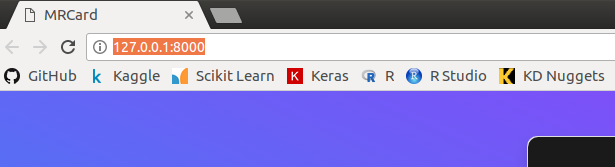
\includegraphics[width=\linewidth]{img/url.png}
		\end{figure}

		Input your Annual Income (rough), Age, Gender and Citizenship, they are all required fields. We use this to calculate which Credit Cards you are eligible for.

		\begin{figure}[H]
			\centering
			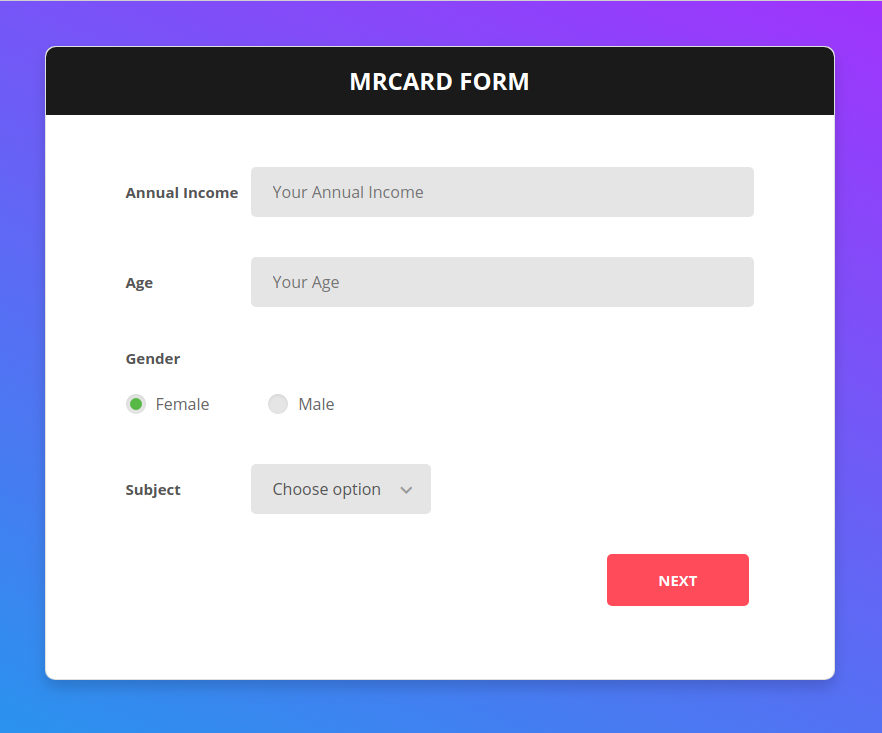
\includegraphics[width=\linewidth]{img/eligibility.png}
		\end{figure}

		Input your Annual Income (rough), Age, Gender and Citizenship are all required fields. If you do not fill in a given field, a prompt will be exposed to remind you.

		\begin{figure}[H]
			\centering
			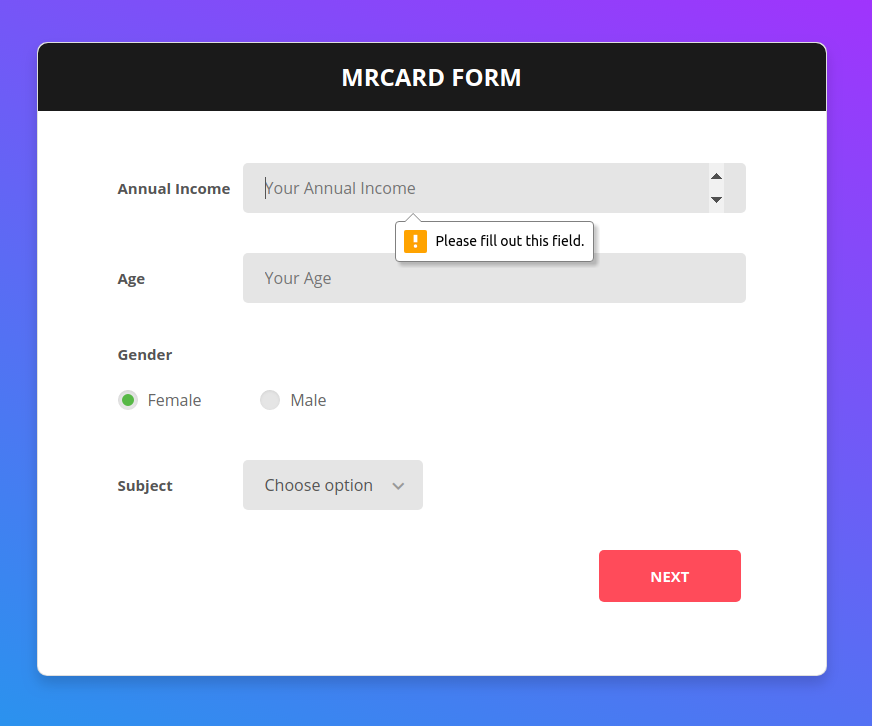
\includegraphics[width=\linewidth]{img/eligibility_fill_in.png}
		\end{figure}

		Next, you get to choose which Bank/ Payment Network and Rewards type you prefer. We will include this as part of the recommendation for preferred cards, together with the ideal Credit Card. From the set of eligible Cards, we recommend an ideal card. And from the set of eligible and preferred Credit Cards, we recommend a preferred card.

		\begin{figure}[H]
			\centering
			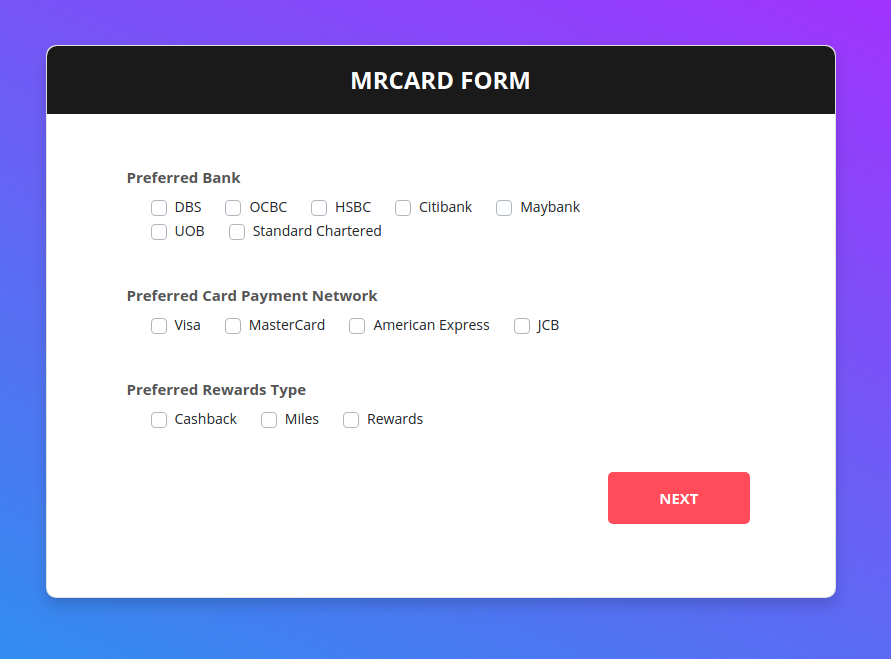
\includegraphics[width=\linewidth]{img/preferences.png}
		\end{figure}

		Following which, click on which categories you spend on with a Credit Card. We use this internally so that we don’t need to ask you unnecessary questions for categories that you don’t spend on. (e.g. If you select Groceries, we will ask you how much you spend on it) We also have a more granular breakdown for certain categories because the breakdown matters when calculating Cashback/ Miles/ Rewards.

		\begin{figure}[H]
			\centering
			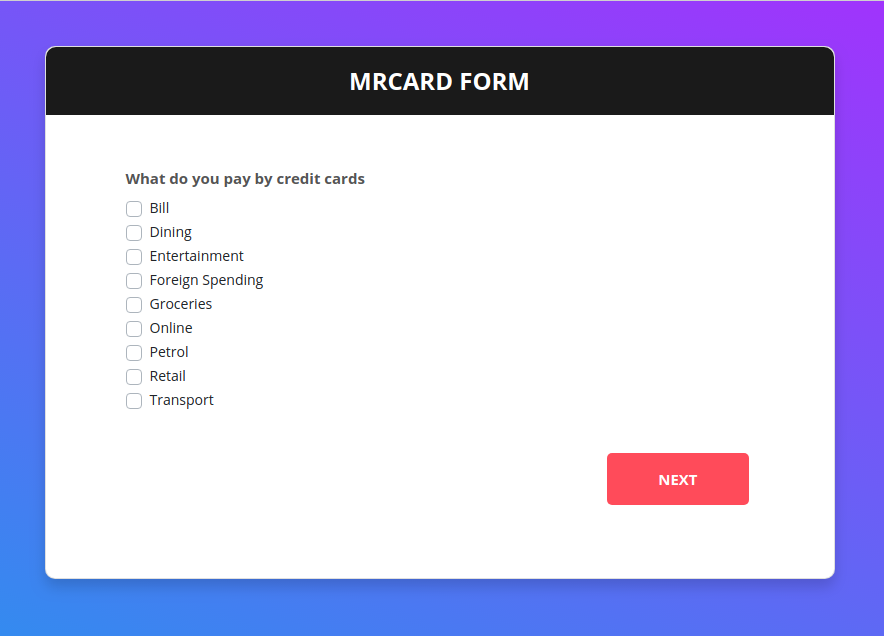
\includegraphics[width=\linewidth]{img/spending_checkbox.png}
		\end{figure}

		Next, please input your spending amounts for each category. You can choose to be as granular as you want or just give a rough estimate (but our calculation will be less accurate then!)

		\begin{figure}[H]
			\centering
			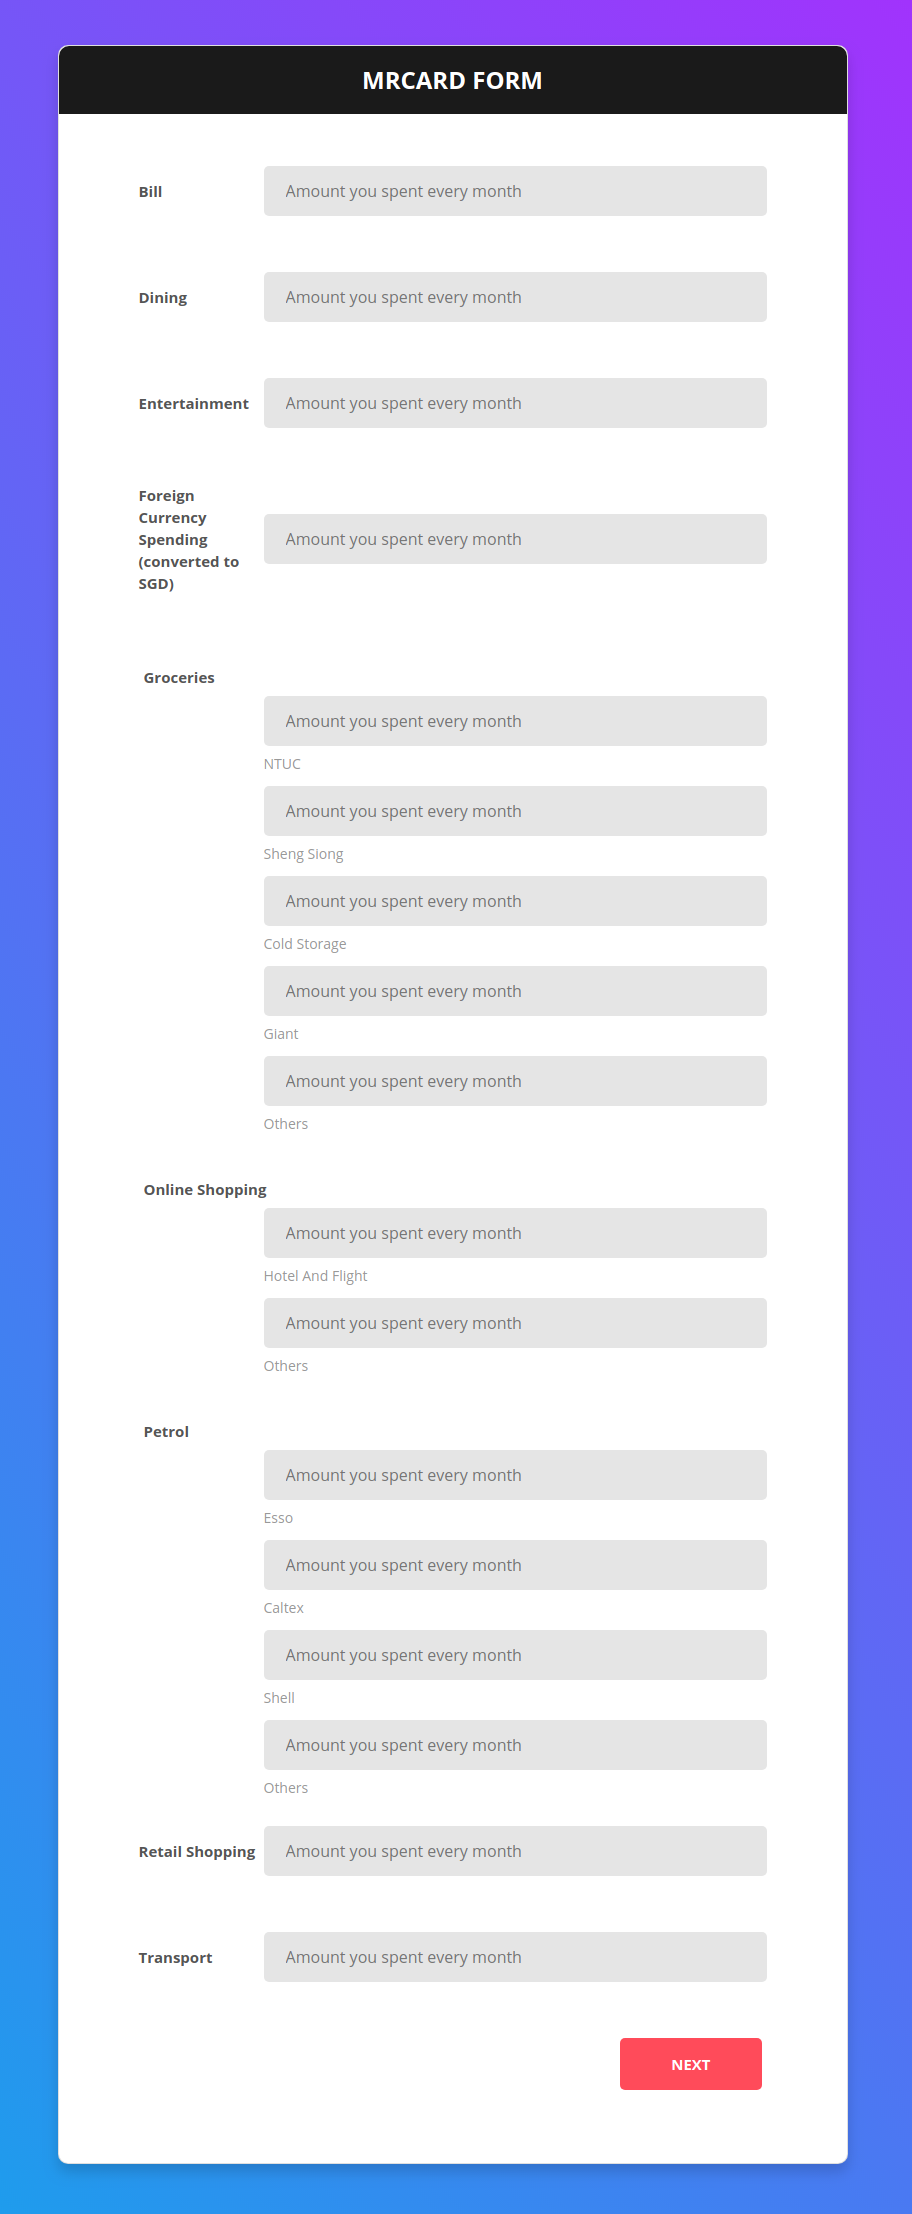
\includegraphics[scale=0.42]{img/spending_amount.png}
		\end{figure}

		And finally based on your eligibility, preferences, spending categories and spending amount, we calculate and give you your recommend ideal and preferred credit card. Click on the Apply button for a link to the official website to sign up! Cheers!

		\begin{figure}[H]
			\centering
			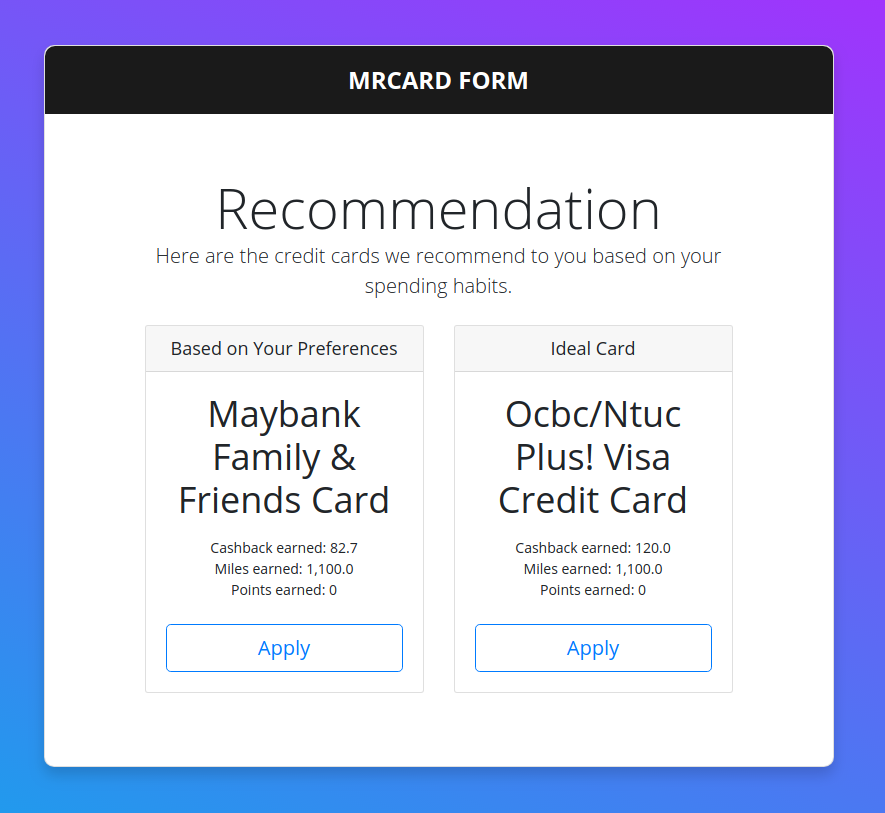
\includegraphics[width=\linewidth]{img/recommendation_v2.png}
		\end{figure}
	% section start (end)


\end{document}
